\documentclass[10pt]{article}

% amsmath package, useful for mathematical formulas
\usepackage{amsmath}
% amssymb package, useful for mathematical symbols
\usepackage{amssymb}

% graphicx package, useful for including eps and pdf graphics
% include graphics with the command \includegraphics
\usepackage{graphicx}

% cite package, to clean up citations in the main text. Do not remove.
\usepackage{cite}

\usepackage{color} 

% Use doublespacing - comment out for single spacing
\usepackage{setspace} 
\doublespacing

% Text layout
\topmargin 0.0cm
\oddsidemargin 0.5cm
\evensidemargin 0.5cm
\textwidth 16cm 
\textheight 21cm

% Bold the 'Figure #' in the caption and separate it with a period
% Captions will be left justified
\usepackage[labelfont=bf,labelsep=period,justification=raggedright]{caption}

% Use the PLoS provided bibtex style
\bibliographystyle{plos2009}

% Remove brackets from numbering in List of References
\makeatletter
\renewcommand{\@biblabel}[1]{\quad#1.}
\makeatother


% Leave date blank
\date{}

\pagestyle{myheadings}
%% ** EDIT HERE **

\usepackage{multirow}

%% ** EDIT HERE **
%% PLEASE INCLUDE ALL MACROS BELOW

% figure files reside in the figures/ directory
\graphicspath{
{figures/}
}

%% END MACROS SECTION

\begin{document}

% Title must be 150 characters or less
\begin{flushleft}
{\Large
\textbf{Spatially explicit model of the lymphocyte diaspora in influenza-infected lung reveals thresholds on chemokine directed migration (SUPPLEMENT)}
}
% Insert Author names, affiliations and corresponding author email.
\\
Drew Levin$^{1,\ast}$, 
Stephanie Forrest$^{1}$, 
Soumya Banerjee$^{1}$,
Candice Clay$^{2}$, 
Melanie Moses$^{1}$, 
Frederick Koster$^{1,2}$
\\
\bf{1} Department of Computer Science, University of New Mexico, Albuquerque, NM, USA
\\
\bf{2} Lovelace Respiratory Research Institute, Albuquerque, NM, USA
\\
$\ast$ E-mail: Corresponding drew@cs.unm.edu
\end{flushleft}


% You may title this section "Methods" or "Models". 
% "Models" is not a valid title for PLoS ONE authors. However, PLoS ONE
% authors may use "Analysis" 
\section{Models}

\subsection{T Cell Production Rate}

We calculate the rate of production ($\sigma$) of CD8 T cells using a differential equation model from \cite{Miao2010}.  The equations model T cell production and subsequent search over an area of infected lung tissue.

{\footnotesize
\begin{equation*}
\label{EqS1}
\begin{aligned}
\dot{N_{c}} &= \sigma - \frac{r'^{2} \cdot N_{c}}{R^{2} \cdot t_{rc}}    & \pi r'^{2} &= a \sqrt{I} + b \\
\dot{N'_{f}} &= \frac{(r'^{2} - r^{2}) \cdot N_{c}}{R^{2} \cdot t_{rc}} - \frac{v_{tcell}}{(r' - r) / 2} \hspace*{2cm}  & \pi r^{2} &= \pi r_{cell}^{2} \cdot I \\
\dot{N_{f}} &= \frac{r^{2} \cdot N_{c}}{R^{2} \cdot t_{rc}} + \frac{v_{tcell}}{(r' - r) / 2} \\
\dot{T} &= \rho T -\beta TV \\
\dot{I} &= \beta TV - \delta I - k_{e} N_{f} I \\
\dot{V} &= pI - \beta TV - \gamma (t) V \\
\gamma (t) &= \left\{ \begin{array}{rcl}
	1/\mbox{day} & \mbox{,}  & t < 5  \\
	3/\mbox{day} & \mbox{,} & t \geq 5  
	\end{array}\right. \\
\end{aligned}
\tag{S1}
\end{equation*}
}
\vspace{.05in}

$N_{c}$ is the number of circulating activated antigen-specific CD8 T cells, $N'_{f}$ is the number of circulating T cells that have found and exit into a region of lung tissue expressing chemokines, $N_{f}$ is the number of circulating T cells that have found an infected region. $T$ is the number of uninfected \textit{target} cells, $I$ is the number of productively infected cells, and $V$ is the viral titer in serum. The infected region is assumed to be of radius $r$ and is within a region expressing chemokines of radius $r'$ ($r  < r'$). The lung is modeled as a circular region with radius $R$. The area of the infected region is equal to the area of an infected cell (of radius $r_{cell}$) multiplied by the number of infected cells. See Fig. 1 for more details about the model.  The area of the region expressing chemokine was found to be related non-linearly to the number of infected cells ($\pi r'^{2} = a \sqrt{I} + b$) where $a$ and $b$ are constants that depend on the viral strain.  $a$ and $b$ were fit using 12 experimental runs of a spatial model implemented in CyCells.

Circulating CD8 T cells ($N_{c}$) are assumed to be released from lymph nodes at a constant rate $\sigma$ and circulate to the $N'_{f}$ population over a time defined by $t_{rc}$. These circulating cells transition into $N'_{f}$ and $N_{f}$ at rates proportional to the areas of the chemokine expressing and infected regions relative to the whole lung area. 

The average time an exiting CD8 T cell takes to migrate is proportional to the difference in the radii between the two regions ($r' - r$) at a given speed, $v_{tcell}$.  Circulating cells that are in the chemokine expressing region ($N'_{f}$) transition to the infected region after walking randomly for that time. Target cells ($T$) become infected by virus at rate $\beta TV$, where $\beta$ is the rate constant characterizing infection. Infected cells ($I$) die at rate $\delta$ in addition to being lysed by T cells ($N_{f}$) at a rate $k_{e}$. Finally the viral titers ($V$) increase due to production of virus at rate $p$ by infected cells. Virus is also cleared due to uptake by infected cells (at a rate $- \beta TV$) and due to antibody (at a rate $\gamma (t)$ that changes after 5 days post infection). The initial viral titer was initialized to 10,000 PFUs and the initial number of target cells was one million. The initial number of infected cells is assumed to be zero. Parameter values are listed in Table S1 in Text S1.  This ODE was fit to data taken from \cite{Miao2010} using Matlab's \texttt{nlinfit} function in order to obtain a value for $\sigma$.  The final value was found to be 777 per hour.


\subsection{CyCells Implementation Details}

The CyCells modeling environment splits its populations into two types: cells and molecules.  Cells are considered to be unique agents and are modeled individually.  On the other hand, molecules are considered to be too small and numerous to model explicitly and are thus represented as compartmentalized concentrations.  These compartments are arranged as a grid that covers the environment.  Each square in the grid contains a unique concentration of the given molecule.  Multiple molecules are represented in separate grids.

Molecular behavior is limited to diffusion and decay.  At each time step, CyCells decreases the concentration of each square in the grid according to the decay rate specified for the given molecule.  CyCells then diffuses the molecules by applying a discrete diffusion equation to each grid square, taking into account the specified diffusion constant and the concentrations in neighboring squares.

New molecules can be secreted by cell objects, such as an infected cell secreting new virus.  In this scenario CyCells calculates the amount of virus secreted per time step, based upon the cell's defined production rate, and then adds this quantity to the grid square that overlaps the secreting cell.  If a cell wants to remove molecular concentration, it will subtract from the square it overlaps.  If the concentration at that square is not enough, concentration will be removed from neighboring squares in an ever expanding diamond.

To model cell dependence on the local molecular concentration, the cell will measure the local concentration at its position by calculating a linearly interpolated combination of the concentrations in the grid squares surrounding the cell.


\subsection{Model Implementation Details}

An overview of the model implementation is shown in Fig. 2.  The model is initialized with one virus-secreting cell placed in the middle of a 2-dimensional sheet of hexagonally-tiled epithelial cells (46,085 total cells).  The sheet measures 10$mm$ per side, which is large enough to contain the infection (Fig. 5).  The molecular grid (Text S1 1.2) is initialized with a resolution of 50$\mu m$.  Each time step of the model represents 10 seconds.

Healthy cells transition to virus-incubating based on a probability that scales linearly with the local virus concentration.   When a cell `becomes infected' it removes the amount of viral concentration equal to a single virion. 

Virus-incubating cells idle for 10 hours (with standard deviation $\sigma=1$ hour) and then transition to virus-secreting cells.  Virus-incubating cells also begin to secrete chemokine after 8 hours (except for aH5N1 which only secretes RANTES after a 16 hour delay).  

Virus-secreting cells secrete both virus and chemokine (the RANTES portion of the chemokine production is added in 16 hours after the initial infection) and die after 1,000 minutes of production (16.7 hours).  Virus-secreting cells will also probabilistically transition to apoptizing cells in the presence of T cells (defined by the existence of a T cell within 5$\mu m$).  The number of T cells in the vicinity of the virus-secreting cell has no effect on the rate that apoptosis is induced in the model.

Apoptizing cells secrete virus and chemokine for one hour and then die.

T cells are added to the model at a constant rate of 777 per hour (Text S1 1.1) through a global `oracle' cell that represents the lymph node.  Because the model environment is only a small portion of the entire lung (1\%), most of the T cells miss the model window and are not visually represented.  The T cells that miss enter a dormant searching state and transition to recirculating after a 10 minute delay.  The cells that enter the model window are placed at a random position and begin a random walk.  At each step, these searching cells check the local chemokine concentration.  If the concentration is above the sensitivity threshold, the T cells immediately transition to the chemotaxing state.  If not, searching T cells transition to the recirculating state and are removed from the model window.  Searching and recirculating T cells have a probabilistic decay rate that corresponds to a 3 day lifespan.

Recirculating T cells are not visually represented.  These cells are individually tracked for 6 minutes, after which they are reintroduced as new searching cells with a new chance of entering the model window.

Chemotaxing T cells move directly up the chemokine gradient until they find a local maximum.  T cells probabilistically decay at a rate corresponding to a 2 hour lifespan.  Chemotaxing T cells have no effect other than inducing apoptosis in virus-secreting cells by proximity.



% Results and Discussion can be combined.
\section{Results}

\subsection{Stochastic modeling effects}

Unlike ODE models, which are deterministic, stochastic models such as CyCells can produce different results on different runs (Fig.~S\ref{fig:variance}).  To test the strength of this effect, we ran each model fifty times using the default parameters given in Table 2.  $R^2$ values were calculated for individual runs versus the average of all runs.  The $R^2$ ($\pm$ one standard deviation) for pandemic, seasonal, and avian influenza are: (0.994 $\pm$ .003), (0.986 $\pm$ 0.011), and (0.917 $\pm$ 0.073) respectively.

Each run took the calculated viral production and chemokine production rates for the three different strains of influenza as input and reported the total number of infected cells, including incubating, virus secreting and apoptotic, but not including dead cells.  Therefore the figures approximate plaque growth over time.

Overlaying multiple runs on a single plot reveals a slight growth rate transition 3 days p.i., which reflects the addition of IgM.  In addition, for each infection the number of infected cells declines quickly at day five due to the T cell response. 

The three strains show different levels of virulence, consistent with the results found in \cite{Mitchell2011} (Fig.~S\ref{fig:variance}).  The rapid production of the pandemic H1N1 virus prevents the immune response from containing the infection.  Because pH1N1 is replicates at such a rapid rate, the window of opportunity for T Cells to gain ground is too small.  aH5N1 is cleared completely, sH1N1 is contained but not fully cleared, and pH1N1 recovers and continues to expand.



\subsection{Chemokine combinations}

Because aH5N1 has been shown to suppress the production of interferon \cite{Mitchell2011}, we hypothesize that it renders IP-10 ineffectual.  We hypothesize that this leads to the elevated RANTES secretion rates measured in aH5N1 compared to the other two strains (Table 3).  Because of this behavior IP-10 was not included in the aH5N1 model runs. 

T cell sensitivity depends on receptor density \cite{Desmetz2006} and this was assumed to be constant.  Thus, the chemokines in combination work additively in our model. 

Four models runs (both, IP-10, RANTES, and none) were performed for sH1N1 and pH1N1 strains and two runs (RANTES and none) for  aH5N1.  The runs show how the presence and/or absence of specific chemokines affect the simulated immune response (Fig.~S\ref{fig:chemokine}).  The lack of both chemokines leads to runaway infections in all three strains.  The presence of only RANTES is enough to contain the aH5N1 infection, but is weaker than IP-10 in both H1N1 strains.  In sH1N1 and pH1N1 simulations, IP-10 alone proves to be as effective as the combination of IP-10 and RANTES.  This suggests that RANTES does not play a significant role in infections that stimulate an IP-10 response due to the higher production rates of IP-10.  

% The bibtex filename
\bibliography{references}

\pagebreak

\section*{Figure Legends}

%\begin{figure}[!ht]
%\begin{center}
%%\includegraphics[width=4in]{figure_name.2.eps}
%\end{center}
%\caption{
%{\bf Bold the first sentence.}  Rest of figure 2  caption.  Caption 
%should be left justified, as specified by the options to the caption 
%package.
%}
%\label{Figure_label}
%\end{figure}


%\begin{figure}[ht!]
%\begin{center}
%% 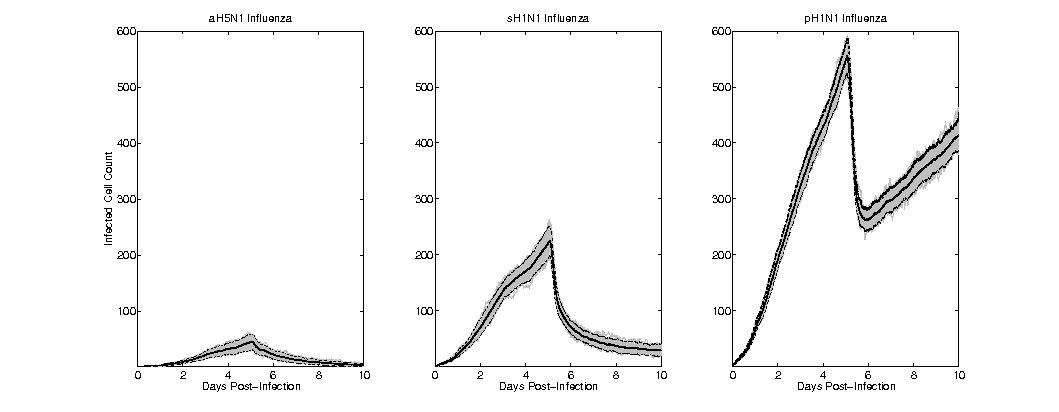
\includegraphics[width=\textwidth]{Figure_S1}
% \end{center}
%\caption{Model results: Time series plots of fifty runs of aH5N1 (A), sH1N1 (B), and pH1N1 (C) infections (gray). IP-10 and RANTES were simulated in each run, except for aH5N1, which  produced only RANTES.  Each run was initialized identically for each strain save for the random seed.  The middle line shows the average while the outer lines show the 95\% confidence interval.} 
% \label{fig:variance}
%\end{figure}
%
%
%\begin{figure}[ht!]
%\begin{center}
%%	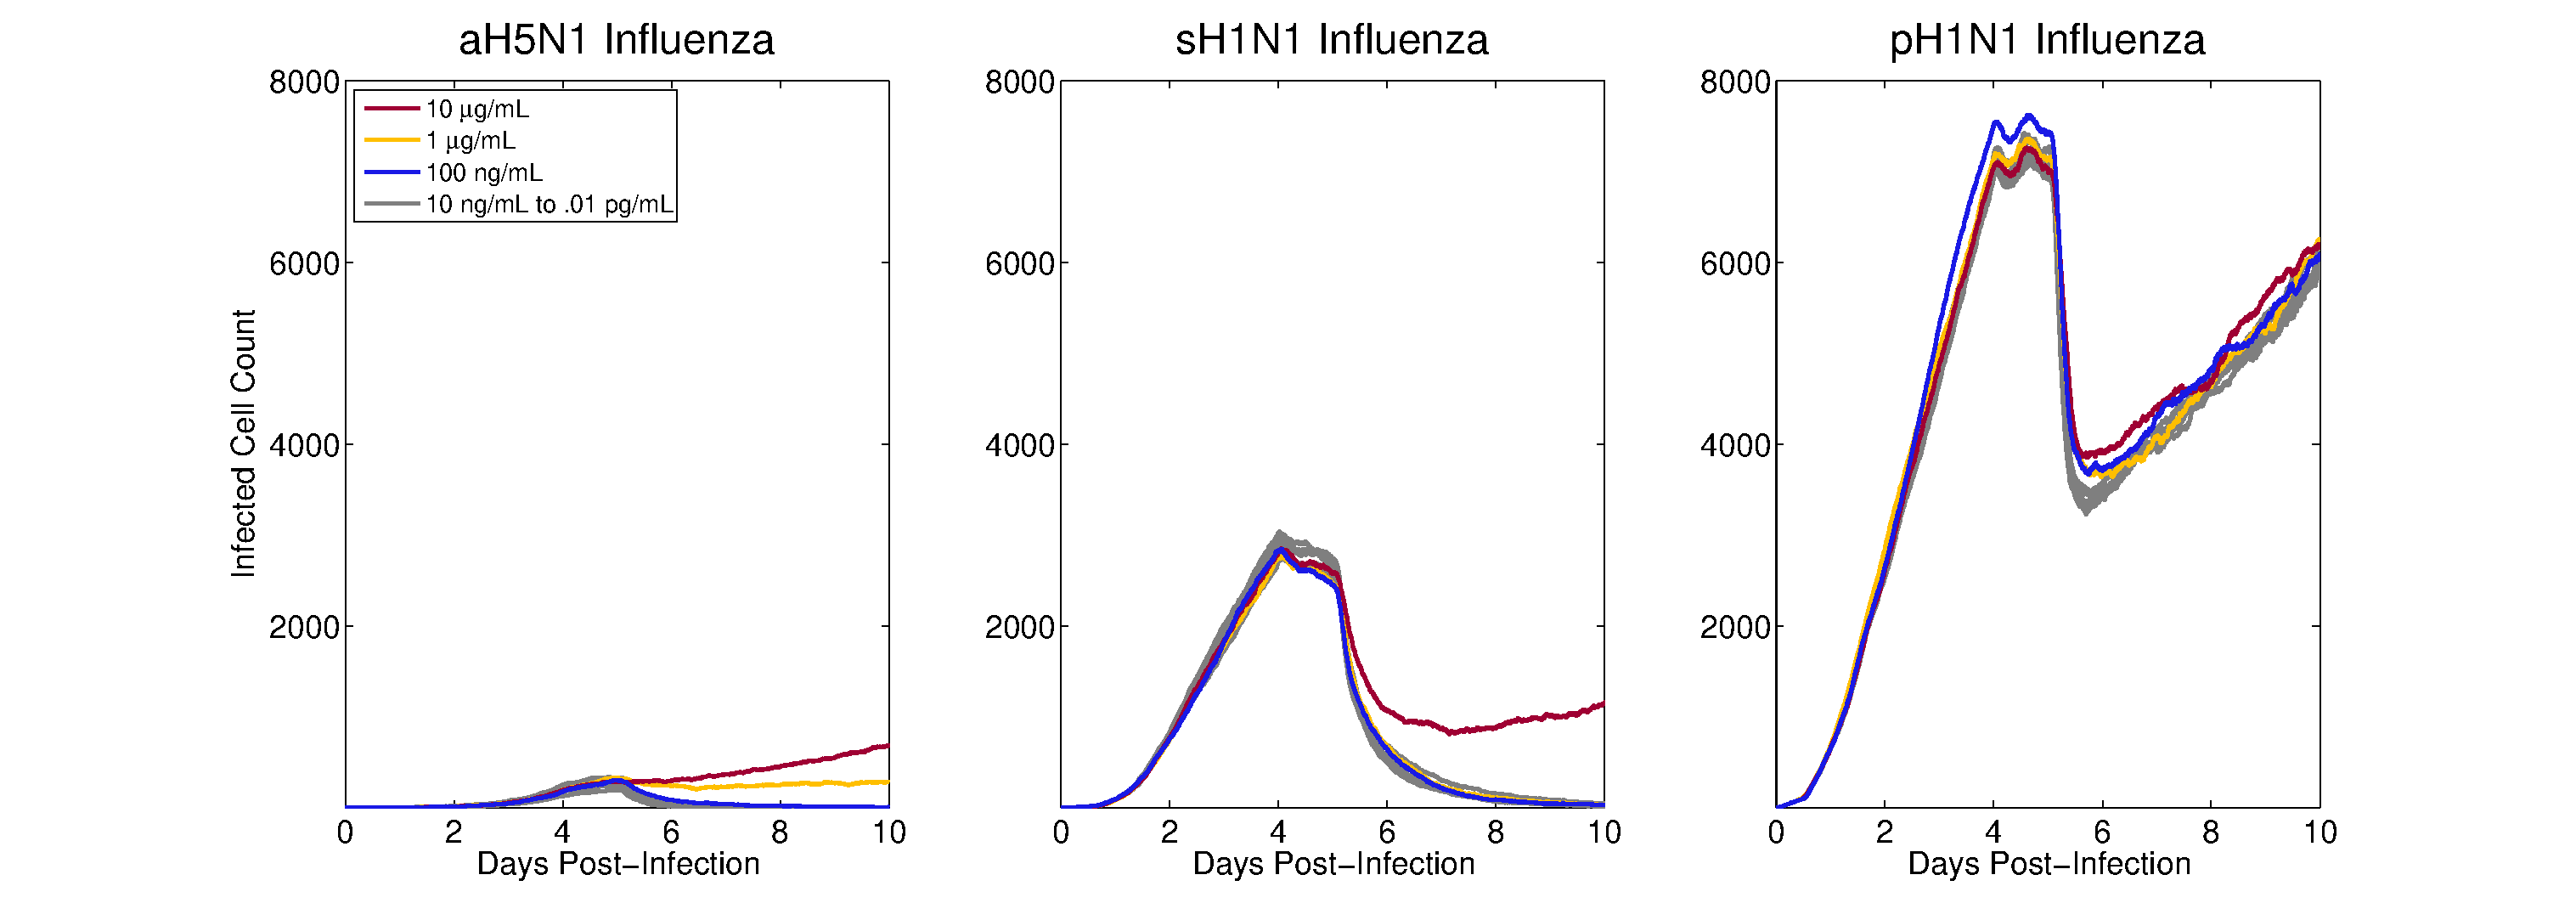
\includegraphics[width=\textwidth]{Figure_S2}
%	\caption{Effects of different chemokine combinations.  A) aH5N1 does not stimulate an IP-10 response.  B-C) sH1N1 and pH1N1 show no significant difference between IP-10 alone versus IP-10 and RANTES combined.}
%	\label{fig:chemokine}
%\end{center}
%\end{figure}
%
%
%\begin{figure}[ht!]
%\caption{The first of three overlaid videos of a representative seasonal H1N1 infection.  This video spans the 10 day infection and shows the cells as they transition from healthy to infected to dead.  T cells show half way through the simulation.  Healthy cells are gray, virus-incubating cells are yellow, virus-secreting cells are orange, apoptotic cells are red, and T cells are green.} 
% \label{video:cell_view}
%\end{figure}
%
%\begin{figure}[ht!]
%\caption{The second of three overlaid videos of a representative seasonal H1N1 infection.  This video spans the 10 day infection and shows the virus concentration.  Notice the volatility when T cells arrive halfway through the simulation.  Virus concentration ranges from 1e-13 mols/mL (white) to 1e-27 mols/mL (black).  Refer to Figure 5 for the detailed legend. } 
% \label{video:virus_view}
%\end{figure}
%
%\begin{figure}[ht!]
%\caption{The third of three overlaid videos of a representative seasonal H1N1 infection.  This video spans the 10 day infection and shows the chemokine concentration.  Notice the volatility when T cells arrive halfway through the simulation.  Chemokine concentration ranges from 1e8 ng/mL (white) to 1e-6 ng/mL (black).  Refer to Figure 5 for the detailed legend. } 
% \label{video:chemokine_view}
%\end{figure}
%
%\begin{figure}[ht!]
%\caption{A closer look at the 2009 pandemic simulation.  This video shows the infection from day 6 to day 7 with each frame spanning 100 simulated seconds.  Healthy cells are gray, virus-incubating cells are yellow, virus-secreting cells are orange, apoptotic cells are red, and T cells are green.  Note the high proportion of virus-secreting cells (orange) early on.  As time passes, secreting cells are gradually contained to the point where they become very sparse.  T cell clumping often prevents the T cells from quick discovery of new secreting cells.}
%\end{figure}

\pagebreak

\section*{Tables}

%\begin{table}[!ht]
%\caption{
%\bf{Table title}}
%\begin{tabular}{|c|c|c|}
%table information
%\end{tabular}
%\begin{flushleft}Table caption
%\end{flushleft}
%\label{tab:label}

% \end{table}

\renewcommand{\thetable}{S\arabic{table}}

\begin{table}[!ht]
\begin{center}
\begin{tabular}{ | c | c | c | }
  \hline                        
  Paramter & Value & Source \\
  \hline
  T(0) & $1e6$ & \cite{Mitchell2011} \\
  V(0) &  $1e4$ & \cite{Mitchell2011} \\
  $r_{cell}$ &  $10 \mu m$ & \cite{Miao2010} \\
  $t_{rc}$ & $6s$ & \cite{Peters1983} \\
  $v_{tcell}$ & $0.3 \mu m/s$ & \cite{Miller2003} \\
  $k_e$ & $6.4e-5/cell/day$ & \cite{Miao2010} \\
  $\beta$ & $4.8e-7/cell/PFU$ & \cite{Mitchell2011} \\
  $p$ & $0.18 PFU/h$ & \cite{Mitchell2011} \\
  $\delta$ & $16.7 hours$ & \cite{Mitchell2011} \\
  $a$ & $20.9$ & ABM fits \\
  $b$ & $70.8$ & ABM fits \\
  \hline  
\end{tabular}
\caption{Supplemental model parameters.  Most values are chosen to match the equations borrowed from both \cite{Mitchell2011} and \cite{Miao2010}.  Values \textit{a} and \textit{b} were fit to multiple runs of a simplified CyCells ABM.}
\label{table:supplement}
\end{center}
\end{table}


\end{document}
